 \section{The Design of Safe and Effective Closed-loop Medical Devices}
The design of safe, bug-free, and efficient medical device software is challenging, especially in implantable devices that directly control and actuate partially understood organs. However, such design is also essential; safety recalls of pacemakers and implantable cardioverter defibrillators between 1990 and 2000 affected over 600,000 devices~\cite{recalls}. Importantly, 41\% of these recalls were due to software issues~\cite{medstats1}. 
According to the US Food and Drug Administration (FDA), in 1996, 10\% of \emph{all} medical device recalls were caused by software-related issues. This percentage rose to an average of 15\% of recalls from 2008 to 2012. 
 And, surprisingly given these numbers, there is currently no formal methodology or open experimental platform to test the correct operation of medical device software within the \emph{closed-loop} context of the patient~\cite{killedbycode}. Unlike other industries such as aviation and automotive where the safety concern is focused on a well-defined physical plant~\cite{autosar,AVSI}, in the medical device domain patient response is complex and nondeterministic. As a result there are no well-established standards for the development of medical device software that directly control and actuate the patient. For device manufacturers, this has prompted recent interest in applying formal modeling~\cite{hcmdss, challenge2, challenge3} and verification techniques in medical devices software development~\cite{med-form2,med-form1}.\vspace{4pt}
 
\emph{How do you guarantee the device software will not adversely affect the patient under all physiological conditions?}

%problems with testing and need for FM approach
~An effective software verification methodology is therefore needed for the risk analysis and certification of medical device software during the FDA's pre-market submission phase. Testing medical device software currently is ad hoc, open loop, and very expensive~\cite{testing_imd, Vip}. Test generation must be interactive and adaptive and must consider the current state of the patient when generating the next input in a way that advances the purpose of the test. The problem, therefore, becomes one of controller synthesis and cannot be addressed by an off-the-shelf model checker~\cite{rushby}. The key challenge is in the generation of \emph{physiologically relevant} software that does not provide inappropriate therapy or adversely affect the patient. This requires validated patient models of the appropriate abstraction levels and that testing is conducted within the closed-loop context of the patient model.

%building blocks - closed-loop, modeling->synthesis, integrated models, translation
Consequently, there is a need for fundamentally novel approaches to the closed-loop modeling, analysis, and design of medical cyber-physical systems, as well as the development of holistic, heterogeneous physiological models, approaches, and tools that address the many different physical, functional and logical aspects of the device and patient interaction. The scientific agenda of this research on medical cyber-physical systems is to unify theories of formal methods, control of physiological systems, communication and computing systems. Our early efforts are conducted with implantable medical devices, such as cardiac pacemakers and defibrillators, and physiological control systems such as infusion pumps with networks of discrete sub-systems. Both feature tight coupling with the patient-in-the-loop, exposing safety and efficacy risks of autonomous and automatic control of the body.\vspace{4pt}

%focus 1
\textbf{1. Implantable Medical Devices - Cardiac Pacemakers:}
~The human heart is perhaps the most important real-time system, generating electrical impulses that determine the heart's rhythm and proper function. Irregularities with timing, i.e. cardiac arrhythmias, cause inefficient and unsafe function of the blood-oxygen system, necessitating the maintenance of the heart rate artificially. The cardiac pacemaker is a rhythm management device that maintains the minimum heart rate and  synchrony between its chambers, thereby improving the condition of patients with cardiac arrhythmias. Cardiac rhythm management devices have grown in complexity with over 80,000 to 100,000 lines of code~\cite{pauljones}. The primary approach to system-level testing of medical devices is unit testing using a playback of pre-recorded electrogram and electrocardiogram signals. This tests if the input signal triggers a particular response by the pacemaker but cannot evaluate if the response was appropriate for the patient condition. Furthermore, this approach of {\em open loop} ``tape testing'' is unable to check for safety violations due to inappropriate stimulus by the pacemaker. Pacemaker Mediated Tachycardia (PMT), a condition where the pacemaker inappropriately drives the intrinsic heart-rate toward the maximum rate, is a strong example of why we need an interactive and adaptive {\em closed-loop} verification and testing of such systems. With a tape test, PMT would not be observed and the response of the pacemaker could be classified as appropriate therapy.
%%%%%%%%%%%%%%%%%%%%%%%%%%%%%%%%%%%%%%%%%%%%%%%%%%%%%%
\begin{figure}[t]
	\centering
	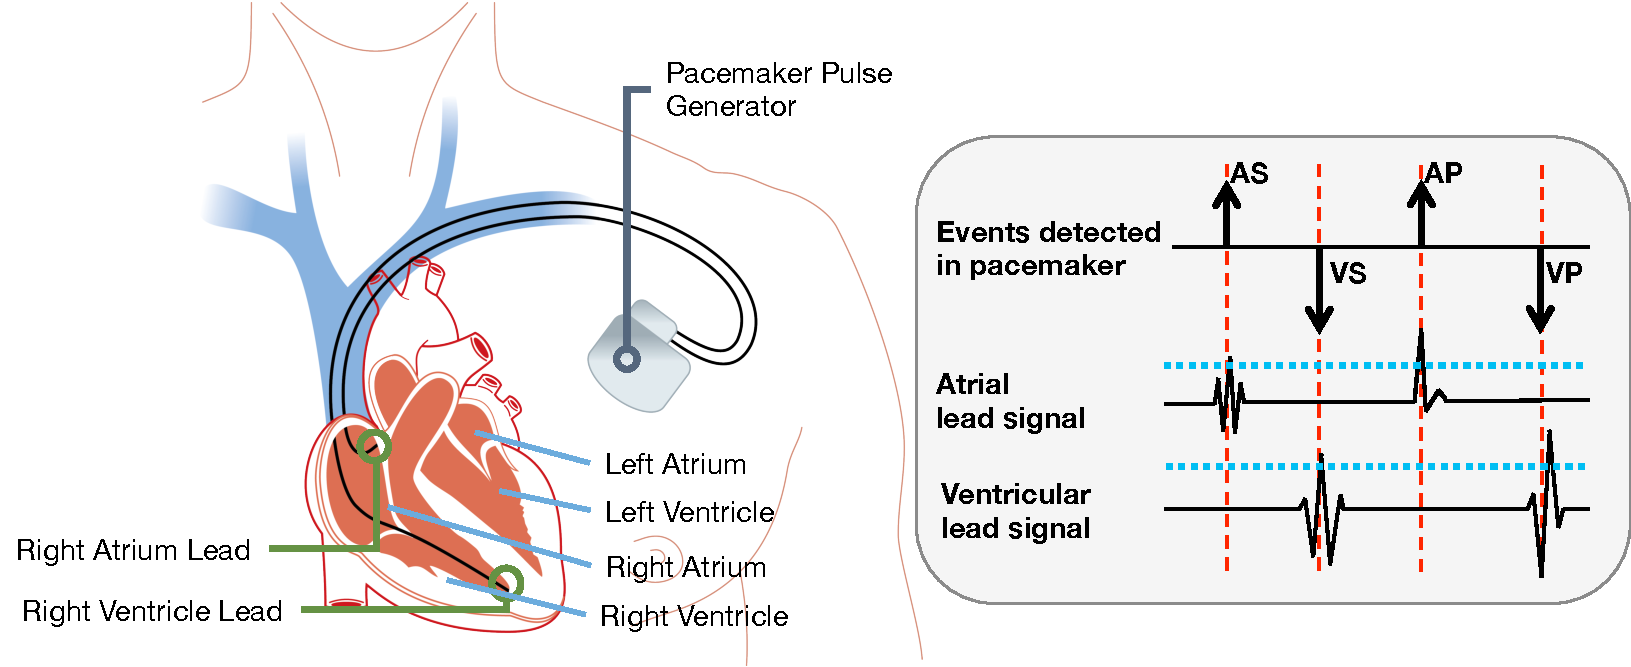
\includegraphics[scale=0.33]{figs/fig1pacemaker.pdf}
	\caption{\small Pacemaker operating in a closed-loop with the heart. The leads sense cardiac electrophysiological activity from inside the heart tissue (AS/VS = Atrial/Ventricular Sense event) and actuate the heart (AP/VP = Atrial/Ventricular Pacing event to maintain the heart rate.}
	\vspace{-20pt}
	\label{fig:pacemaker}
\end{figure}
%%%%%%%%%%%%%%%%%%%%%%%%%%%%%%%%%%%%%%%%%%%%%%%%%%%%%%
\begin{figure}[!b]
	\centering
	\vspace{-20pt}
	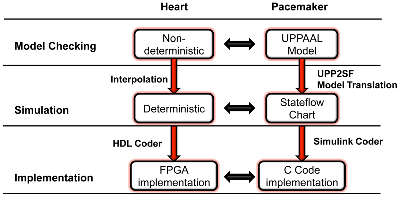
\includegraphics[scale=1.2]{figs/model_based_b.pdf}
	\caption{\small From closed-loop verification to simulation-based testing, code generation and platform evaluation}
	\label{fig:med_overview}
\end{figure}
%%%%%%%%%%%%%%%%%%%%%%%%%%%%%%%%%%%%%%%%%%%%%%%%%%%%%%
%%%%%%%%%%%%%%%%%%%%%%%%%%%%%%%%%%%%%%%%%%%%%%%%%%%%%%
\begin{figure*}
	\centering
	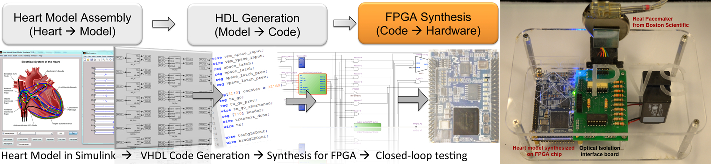
\includegraphics[scale=1.4]{figs/pvs_toolchain.pdf}
	\caption{\small From verified models to verified code: Translating models to a heart-on-a-chip platform for closed-loop testing of cardiac devices}
	\vspace{-10pt}
	\label{fig:pvs_toolchain}
\end{figure*}
%%%%%%%%%%%%%%%%%%%%%%%%%%%%%%%%%%%%%%%%%%%%%%%%%%%%%%

Our proposed model-based design (MBD) for Medical CPS begins with developing integrated functional and formal heart models that interact with real and modeled pacemakers for closed-loop verification and testing~\cite{vhm_proc}. As shown from the top of \figref{med_overview}, the heart-pacemaker closed-loop systems is first modeled abstractly to facilitate verification of the basic pacemaker design with maximum coverage~\cite{vhm_tacas12}. In our case, we use timed automata~\cite{timed_automata, timed-aut} and the UPPAAL model checker~\cite{BDL04, uppaal, uppaal_tut} at this design stage. Next, the models are translated to more detailed models that take into account the complex dynamics of the heart and interaction with more detailed pacemaker model~\cite{vhm_ecrts10, vhm_embc11,vhm_iccps11}. We use Stateflow and Simulink~\cite{stateflow, volkswagen} at this design stage. These models are validated by physicians for their clinical relevance. The automatic model translation procedure, from UPPAAL to Stateflow, ensures that abstract models used for verification over-approximate the more detailed models used downstream~\cite{vhm_rtas12}. Once the detailed models pass simulation-based testing with closed-loop dynamics, they are automatically generated into code and are subject to platform-level integration testing~\cite{vhm_website} as shown in \figref{pvs_toolchain}. This MBD approach ensures the closed-loop safety properties are retained through the design toolchain and facilitates the development of verified software from verified models.\vspace{4pt}

%focus 2
\textbf{2. Physiological Control Systems:}
~The understanding of closed-loop safety analysis of single-system devices such pacemakers has naturally broadened our work to physiological control systems featuring multiple networked devices with the patient-in-the loop~\cite{pcs_iccps10}. Such a clinical scenario is viewed as a control system, in which the patient is the plant, bedside monitors are sensors and drug infusion pumps are actuators~\cite{hcmdss}.  In this setup, caregivers traditionally perform the role of the controller. In many cases automatic controllers for drug infusion can reduce the burden on the caregiver and avoid human errors. However, vendors of medical equipment continue to avoid closed-loop scenarios due to an insufficient understanding of the human body's response to treatment. Furthermore, a particular challenge arises from the complex interplay between the continuous dynamics of the patient's reaction to treatment, and discrete controller and network. 
%Despite many medical devices being able to send sensed data across the network, only few modern medical devices can be controlled remotely. 
%%%%%%%%%%%%%%%%%%%%%%%%%%%%%%%%%%%%%%%%%%%%%%%%%%%%%%
\begin{figure}[!b]
	\centering
	\vspace{-10pt}
	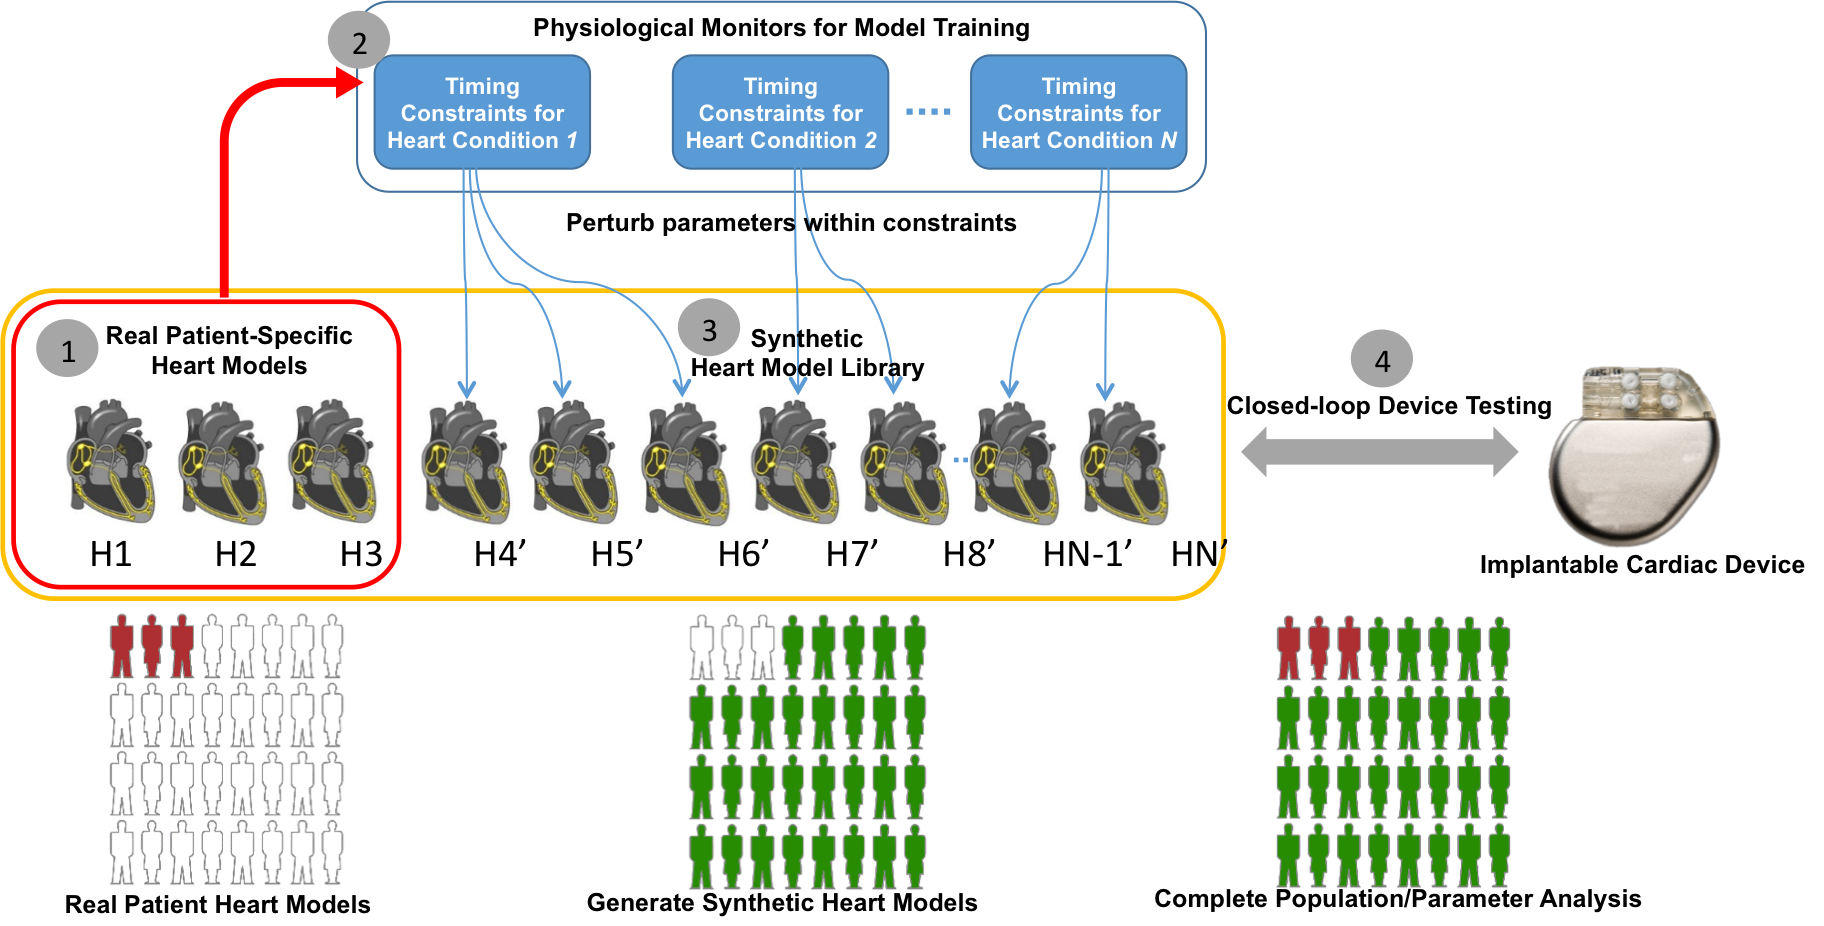
\includegraphics[scale=0.3]{figs/mbct.png}
	\caption{\small Model-based Clinical Trials}
	\label{fig:mbct}
\end{figure}
%%%%%%%%%%%%%%%%%%%%%%%%%%%%%%%%%%%%%%%%%%%%%%%%%%%%%%
Consequently, there is a need for model driven safety analysis of closed-loop medical systems within uncertain parameters. Both the abstract, formal model and the detailed, informal model are needed in the process of verification, validation, and regulatory approval of closed-loop medical device systems.  Formal models allow us to exhaustively explore the possible behaviors of the system and prove its safety, detailed models allow us to use high-fidelity simulation that take real system dynamics into account.  Both kinds of results can be used to make the case for regulatory approval if the abstract model is guaranteed to over-approximate the patient's dynamics with respect to the control algorithms used.\vspace{4pt}

\textbf{3. Model-based Clinical Trials:}
~Regulatory authorities require that the safety and efficacy of a new high-risk medical device be proven in a Clinical Trial (CT), in which the effects of the device on a group of patients are compared to the effects of the current standard of care. 
Phase III trials can run for several years, cost millions of dollars, and pose an inherent risk to the patients by exposing them to an unproven device.
With the use of computational modeling and simulation, we would like to investigate how to use a large model-based synthetic group of patients and device models to improve the planning and execution of a CT so as to increase the chances of a successful trial.

As an example, we apply our initial efforts are in applying it to a real CT that compares two algorithms within implantable cardioverter defibrillators (ICDs) for the detection of potentially fatal cardiac arrhythmias~\cite{RIGHT}. 
In 2011, a CT posited that one algorithm (Boston Scientific's) would be better than the other (Medtronic's) but the results of the trial were opposite to this hypothesis~\cite{RIGHTresults}. 
We begin by modeling the heart and processing 100's of real patients' electrogram signals, mapping the timing and morphology components of the signals to the heart model. 
This is followed by generating a population of 10,000+ synthetic heart models, by perturbing the parameters of the initial heart models for different arrhythmias, and implementing diagnostic algorithms of two very commonly used ICD platforms in the USA, i.e. Boston Scientific and Medtronic.
We conducted conformance testing to validate our device models against real ICDs. 
Now, using the closed-loop of the device models and synthetic patient population we conducted multiple trials to compare the performance of the two algorithms to appropriately discriminate between potentially fatal ventricular tachycardias (VT) and non-fatal SupraVentricular Tachycardias (SVTs). 

The results of our model-based clinical trials (MBCT) indicate we could have accurately predicted this with our model, i.e. that Boston Scientific's algorithm was less able to discriminate between SVT and VT and so may lead to inappropriate therapy.
We further demonstrated that the result continues to hold if we vary the characteristics of the synthetic population and device parameters.
% - thus indicating that the CT was unlikely to prove the desired effect. 
While MBCTs do not seek to replace a CT, they may provide early insight into the factors which affect the outcome at a fraction of the cost and duration and without the ethical issues.
This effort is an early step towards using computer modeling as regulatory-grade evidence for medical device certification. 

 